\documentclass[a4paper,10pt]{article}
\usepackage[T1]{fontenc} 
\usepackage[utf8]{inputenc}
\usepackage[frenchkw]{algorithm2e}
\usepackage[francais]{babel}
\usepackage{graphicx}
\usepackage{amsfonts}
\usepackage{amsmath}

%opening
\title{}
\author{}

\begin{document}

\maketitle

\begin{abstract}
%a la fin
\end{abstract}

\section{Qu'est ce qu'un système de recommandation?}

\subsection{Notre approche}

Le but de notre projet est de pouvoir recommander un film ou plusieurs à n'importe quel utilisateur. 
Pour cela, nous devons savoir à quel point un utilisateur va aimer tel ou tel film pour le lui recommander ou pas. 
Il nous faut donc une sorte d'échelle d'affinité entre l'utilisateur et chaque film. Ce qui parait pertinent est alors d'estimer pour chaque film une note que lui donnerait l'utilisateur s'il le voyait.
Nous pourrons ainsi recommander le film ayant la meilleur note prédite.
Notre objectif est de trouver un modèle mathématique permettant de déterminer la note que mettrait un utilisateur à n'importe quel film qu'il n'a pas vu. 
Cependant il nous faut nous appuyer sur quelque chose. Pour commencer à travailler, il faut déjà connaître certaines informations : nous travaillerons avec des notes de films données par un certain nombre d'utilisateurs.

\subsection{Première difficulté : les données}
\subsubsection{Extraction des données}

Le besoin d'avoir des données nous guide vers une grande base de données appelée `` movielens '' qui est un site communautaire de recommandation de films où les utilisateurs du site notent des films de 0 à 5.
Plusieurs jeux de données y sont disponibles. 
Nous choisissons de travailler avec des notes données par 670 utilisateurs à 9125 films.
Par la suite nous nous référerons au nombre d'utilisateurs par $n_u$ et au nombre de films par $n_f$.
Nous extrayons alors 2 fichiers : l’un contenant les $n_f$ films avec leurs titres et un numéro d'identification attribué,  
l’autre avec les notes des utilisateurs eux aussi numérotés par des identifiants.
Ce dernier fichier est un tableau avec $n_u$ lignes du type : identifiant de l’utilisateur, id du film qu’il a noté, note. 
Ces 2 fichiers étant peu pratiques pour manipuler leurs données,  
nous créons une fonction tableau\_des\_notes() qui retourne un tableau, une matrice de dimension $n_u * n_f$ qui contient les notes données par les utilisateurs, en ligne, aux films, en colonne. Seulement, aucun utilisateur n'a noté tous les films : il y a des cases vides dans notre tableau. Nous insérons alors dans ces cases des `` NaN ''(Not a Number), type de donnée facile à traiter dans notre programme.
Le tableau des notes est appelé Y.

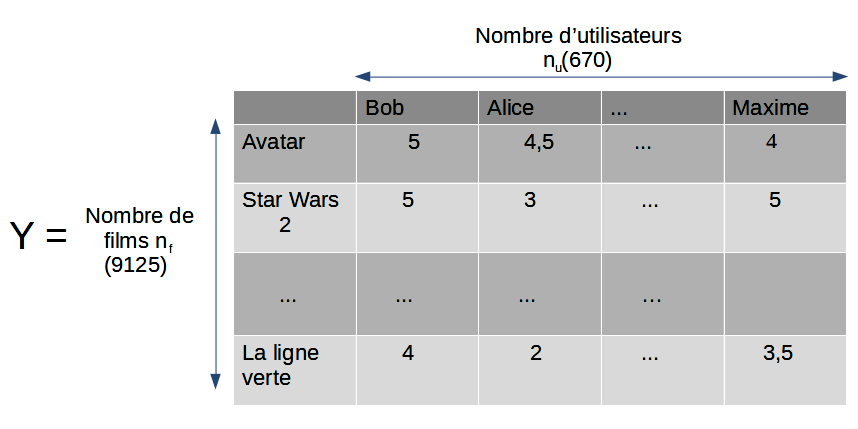
\includegraphics[scale=0.5]{matriceY.png}

\subsubsection{Analyse des données}

Nous créons ensuite deux fonctions permettant de faire des statistiques sur nos données : l’une permettant de compter combien de films chaque utilisateur a vu, et l’autre comptant le nombre de notes attribuées pour chaque film. De ces fonctions, nous tirons des graphiques nous permettant d'avoir une idée plus précise de nos données.\\

Nous remarquons alors que plus de 8000 films possèdent seulement entre 1 et 40 notes, que le plus souvent un film a été noté deux fois et que le film auquel a été attribué le plus de notes a 339 notes.

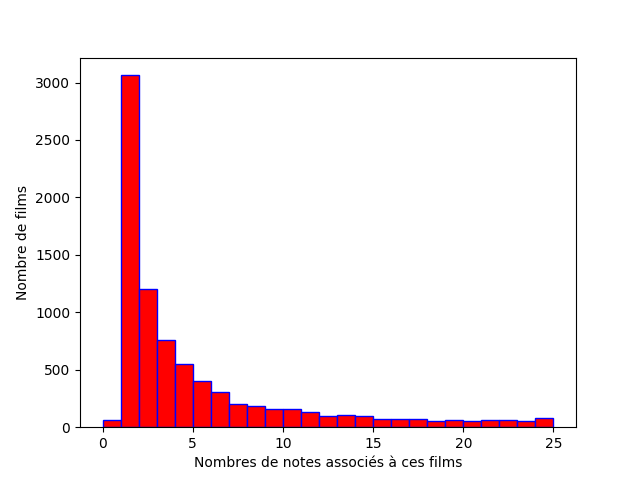
\includegraphics[scale=0.5]{hist2.png}

Dans l’autre sens, nous voyons aussi que chaque utilisateur à noté 148 films en moyenne.

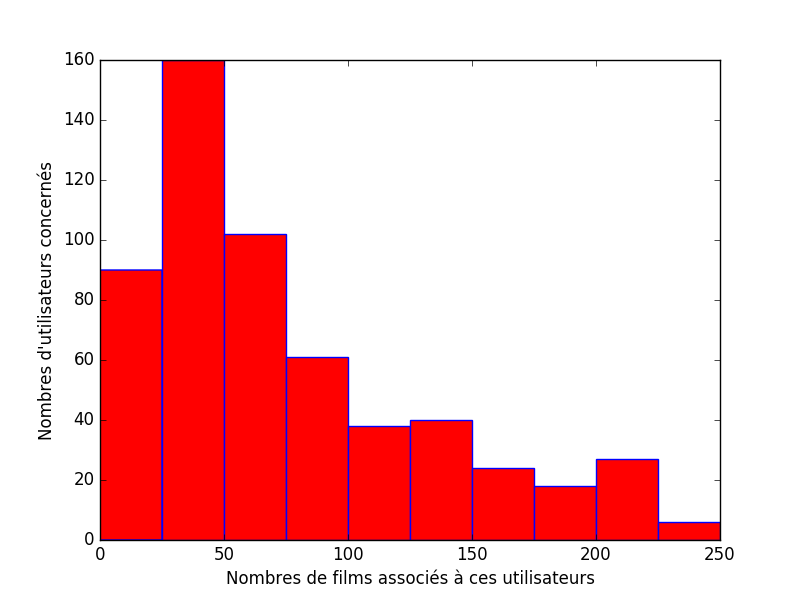
\includegraphics[scale=0.5]{hist1.png}

Autre remarque, notre tableau présente 98,4 \% de NaN.\\

Notre but devient de compléter ces trous, de prédire les notes que nous ne connaissons pas. Alors nous pourrions, en réutilisant la même méthode, pour n'importe quel personne ayant noté quelques films deviner les notes qu'il mettra aux films qu'il n'a pas encore vu.

\section{Formalisation du problème d'optimisation y compris modélisation}

Nous nous posons maintenant la question de comment nous y prendre pour prédire des notes ?
Notre seule ressource est la matrice Y non pleine. Sur quel modèle s'appuyer pour la compléter ?
C'est ce que nous allons étudier dans cette partie.

\subsection{Quelques notations}

Introduisons quelques notations qui seront utilisées par la suite.\\

Nous travaillons tout au long de ce rapport avec des matrices réelles. $\forall (n, p) \in \mathbb{N}^2$ nous notons l'ensemble des matrices réelles de dimension $n * p$ : ${\cal M}_{n, p}$\\
$\forall (n, p) \in \mathbb{N}^2$ $\forall A \in {\cal M}_{n, p}$ $\forall i \in \{1, 2, ..., n\}$ $a_i$ est la i-ème ligne de la matrice A et nous avons $a_i \in {\cal M}_{1, p}$. Et $\forall j \in \{1, 2, ..., p\}$ $a_{., j}$ est la j-ème colonne de la matrice A et nous avons $a_j \in {\cal M}_{n, 1}$. Remarquons que des majuscules sont utilisées pour des matrices qui ne sont ni des matrices lignes ni des matrices colonnes et des minuscules autrement. Nous utilisons aussi des minuscules pour les coefficients des matrices.\\
Sauf indication contraire, lorsque nous utilisons la lettre j il s'agit d'un entier naturel non nul et inférieur ou égal à $n_f$. De la même façon la lettre i représente, lorsque ça n'est pas précisé, un entier naturel non nul et inférieur ou égal à $n_u$.\\
Enfin, le film numéro j est le film dont les notes se trouvent à la j-ème colonne de Y et l'utilisateur i est l'utilisateur dont les notes qu'il a donné sont à la i-ème ligne de Y.

\subsection{Modélisation du problème : factorisation de matrices}

Posons $Y_f$ la matrice Y complétée qui contient toutes les prédictions, exactes, des notes qui nous manquent. C'est la matrice à laquelle nous voulons aboutir, celle que nous devons deviner. Voici notre méthode.\\ 
 
Nous supposons que nous sommes capable de déterminer à partir de Y deux matrices X et $\Theta$ telles que $\Theta X^T = Y_f$ avec $\Theta$ une matrice de dimension $n_u * n$ et X une matrice de dimension $n_f * n$. $n \in \mathbb{N}^*$ est quelconque, nous verrons par la suite que nous pouvons le fixer comme bon nous semble.\\ 
Notre hypothèse sur l'interprétation de $\Theta$ et X ? Ce qui nous fait supposer leur existence ? Nous allons éclairer ce point tout de suite par des explications plus précises.\\

Le paragraphe qui suit est la description de nos suppositions sur l'interprétation que nous pouvons faire à propos de n, $\Theta$ et X. Après chaque verbe au conditionnel il serait possible d'ajouter "d'après notre hypothèse".\\
Parlons un peu du nombre n. Ce dernier serait en fait un nombre de caractéristiques quelconques, qui nous sont inconnues et qui peuvent bien décrire nos films : si nous pensons qu'ils peuvent être décris efficacement par 10 caractéristiques, nous choisissons de trouver $\Theta$ et X avec $n = 10$. 
Une caractéristique peut être n'importe quoi, du taux d'action au taux de blondeur des cheveux de l'actrice principale. Pour l'instant admettons seulement que ces n caractéristiques peuvent exister. Nous les numérotons de 1 à n, puis nous verrons comment elles sont déterminées dans une autre partie.\\
Décrivons X. Nous avons déjà dit que cette matrice possède $n_f$ lignes. Chaque ligne caractériserait un film. Ainsi $\forall j \in \{1, 2, ..., n_f\}$ le film j serait décrit par $x_j$ de dimension $1 * n$. Comment ? En fait $\forall k \in \{1, 2, ..., n\}$ $x_{j,k}$ correspondrait à un taux de correspondance entre le film j et la k-ième caractéristique. Si la k-ième caractéristique est l'action et si le film j est un film d'action tandis que le film j' ($j' \in \{1, 2, ..., n_f\}$) est un film romantique sans action alors $x_{j,k}$ sera un réel supérieur à $x_{j',k}$.\\
Décrivons maintenant $\Theta$. $\forall i \in \{1, 2, ..., n_u\}$ $\theta_{i}$ représenterait les goûts de l'utilisateur i. $\forall k \in \{1, 2, ..., n\}$ $\theta_{i,k}$ serait un taux d'appréciation de la caractéristique k pour l'utilisateur i.\\
Ainsi seraient les deux matrices auxquelles nous voulons aboutir.\\

Voyons maintenant voir en quoi le produit $\Theta X^T$ peut valoir $Y_f$. D'après le produit matriciel, $\forall i \in \{1, 2, ..., n_u\}$ et $\forall j \in \{1, 2, ..., n_f\}$ on a $(y_{f})_{i,j} = theta_{i}(x_{j})^{T}$ : la note que l'utilisateur i a donné ou donnera au film j dépend des caractéristiques du film et du profil de l'utilisateur. Et nous avons :
\[(y_{f})_{i,j} = \sum_{k = 1}^{n} \theta_{i,k} * x_{j,k}\]
Ce qui semble logique : la note est une combinaison linéaire des taux de caractéristiques du film avec des coefficient qui sont plus ou moins élevé suivant le goût de l'utilisateur pour la caractéristique concernée.

\subsection{Fonction de coût}

Nous avons supposé que $\Theta$ et X existent, cependant il est très peu probable que ce soit le cas : nous pouvons arriver à deux matrices avec les dimensions voulues mais avec au mieux $\Theta X^T \approx Y_f$. Notre problème devient alors la minimisation de l'écart entre les notes de $\Theta X^T$ et celles de $Y_f$. Mais nous ne connaissons que quelques notes de $Y_f$ : les notes déjà données par les utilisateurs, celles de Y. Ce qui nous amène à introduire une fonction qui estime un écart entre les notes de $\Theta X^T$ et de Y :
\begin{align*}
J\colon{\cal M}_{n_u, n} \times {\cal M}_{n_f, n} &\longrightarrow \mathbb{R}^+\\
(\Theta, X)&\longmapsto \frac{1}{2}\sum_{\substack{i,j \\ y_{i,j} \ne NaN}}(\theta_{i}(x_{j})^{T}-y_{i,j})^{2}
\end{align*}
Nous appelons J fonction de coût, c'est la fonction à minimiser pour trouver $\Theta$ et X optimaux qui représentent nos données le mieux possible.

\section{Implémentation algo}
%guillaume
\subsection{descente du gradient en general optimisation}
Nous utilisons un algorithme appelé descente du gradient pour minimiser J. Pour illustrer cet algorithme nous allons l'appliquer 
à une fonction $f$ qui dépend de deux variables.%J'aimerai bien mettre la n otation pour une fonction ici
 On a $df = \frac{\partial f}{\partial x_{1}}d x_{1} + \frac{\partial f}{\partial x_{2}}dx_{2}$. En faisant l'approximation
 $\Delta f = \frac{\partial f}{\partial x_{1}}\Delta  x_{1} + \frac{\partial f}{\partial x_{2}}\Delta x_{2}$ on se rend compte
 que en posant $\Delta x_{1} = -\alpha \frac{\partial f}{\partial x_{1}}$
 et $\Delta x_{2} = -\alpha \frac{\partial f}{\partial x_{2}}$ avec $\alpha \in \Re^{+}$
 on obtient $\Delta f = -\alpha \frac{\partial f}{\partial x_{1}}^{2} - \alpha \frac{\partial f}{\partial x_{2}}^{2} < 0$. Ainsi dans
 les limites de l'approximation faite au dessus a chaque fois qu'on modifie les $x_{i}$ de $- \alpha \frac{\partial f}{\partial x_{i}}$
 on a une réduction de $f$.
On applique le même raisonnement sur $J$ avec une subtilité. NOus ne savons pas gerer $\Theta$ et $X$ simultanement. On considere donc une
seul variable l'autre étant supposé constante. Une étape de la descente du gradient a donc deux parties :  on fait varier chaque vecteur caractéristique de chaque film
puis chaque vecteur de préferences de chaque utilisateur.

\begin{algorithm}[H]
 \Donnees{a mettre}  
 \Res{un nouveau x}  
 initialization\;
  \PourTous{j $\in$ \{1, 2, ..., nf\}}{ 
  Affecter à $x_{j}$ la valeur $x_{j}-\alpha \nabla_{x_{j}}J(x, \Theta)$\; 
 }
 \caption{Descente du gradient}
\end{algorithm}
%je sais que c'est trop court et pas assez bien posé mais il faut commencer quelque part
On prouve en \ref{P1} que $ \nabla_{x_{j}}J(x, \Theta) = \nabla_{x_{j}^T}\frac{1}{2}\Vert\tilde{\theta}x_{j}^{T}-\tilde{y}_{.,j}\Vert^{2}$
puis en \ref{P2} on prouve que $\nabla_{x} \frac{1}{2}||Ax - b||^{2}_{2} = A^{T}(Ax - b)$ (Prciser les dimensions et a quoi s'applique ce calcul). ce qui nous permet de dire
que $ \nabla_{x_{j}}J(x, \Theta) =  \tilde{\theta}^{T}(\tilde{\theta}x_{j}^{T}-\tilde{y}_{.,j})$. Ces divers calculs nous permettent
de représenter une étape du gradient comme une série de produits de matrices. Au début, nous devions calculer le résultat terme a terme. Cette
façon de faire était très lente et passer à une représentation matricielle nous a permis de grandement accélérer les étapes de la descente du gradient.
\subsubsection{ecrire algo puis dire comment on a fait au début}
\section{Mise en application de l'algorithme}
\subsection{Familiarisation avec problème plus simple}
Dans la première partie de notre projet, nous avons décidé de simplifier notre problème en extrayant un tableau de données 
plein c'est à dire un tableau où tous les films ont été notés par tous les utilisateurs. 
A partir de ce tableau, nous pouvons donc enlever une note et essayer de la prédire. Ainsi, nous pouvons voir nos erreurs facilement sans avoir à gérer les Nan.
Notre première difficulté a été d'extraire ce tableau plein. Pour cela, l'étude des données faite en amont nous a beaucoup aidé: pour extraire ce tableau ``plein''
nous avons crées une fonction (cf annexe) sélectionnant les films les plus vus puis les utilisateurs qui ont vues tous ces films. On a donc obtenus un
tableau plein 10*11 (10 films pour 11 utilisateurs).
Dans ce cas-ci, nous supposons qu'il existe une relation linéaire commune pour tous les films, c'est à dire que la matrice X serait une matrice colonne.
On fixe donc tout d'abord cette matrice X aléatoirement. Puis on applique la descente du gradient pour trouver les coefficients de cette matrice les plus adaptés.
Ainsi , on peut prédire au mieux une note pour un utilisateur ayant vus tous les films d'avant.
%les trois dernière phrase sont très mal expliquer il faut les reprendre
\subsection{yassine}
\subsubsection{taux d'erreur}
\subsubsection{influence des parametres}
\subsection{limites de notre approche}
%yassine
\subsubsection{Est-ce qu'on arrive a recommander un film a un utilisateur}
%guillaume
Au final une question intéressante est est-ce que le modèle arrivera d'une manière efficace a prédire les notes à un nouvel utilisateur. Pour faire cela nous avons
choisi de ne pas recalculer $X$ et $\Theta$ pour chaque nouvel utilisateur. À la place, nous supposons que l'ajout d'un utilisateur ne va pas modifier
les caractéristiques d'un film. Il nous suffit donc de calculer et d'ajouter une nouvelle ligne seulement à $\Theta$ caractérisant le profil du nouvel utilisateur. Ceci peut alors se faire très rapidement. À partir de ces nouvelles données, il nous suffit de compléter Y pour trouver la note la plus élevée et recommander à l'utilisateur le film associé. Toutefois l'erreur sur la prédiction des notes nous laisse penser que ce film ne serait probablement pas le meilleur film pour cet utilisateur, car le hasard aurait bien pu faire que le meilleur film ait une note plus basse de 1 point ce qui suffirait à lui faire perdre la première place.
\section{Conclusion}
%1 page

\subsection{perspectives}
%guillame
\appendix 
\section{Preuves} 
\subsection{} 
\label{P1} 
$\nabla_{x_{j}^T} J(\theta, X)= 
\begin{pmatrix} 
\displaystyle\frac{\partial \displaystyle\sum_{k=1}^{nf}\frac{1}{2}\Vert\tilde{\theta}x_{k}^{T}-\tilde{y}_{.,k}\Vert^{2}}{\partial x_{j,1}^{T}}\\ 
\displaystyle\frac{\partial \displaystyle\sum_{k=1}^{nf}\frac{1}{2}\Vert\tilde{\theta}x_{k}^{T}-\tilde{y}_{.,k}\Vert^{2}}{\partial x_{j,2}^{T}}\\ 
\vdots\\ 
\displaystyle\frac{\partial \displaystyle\sum_{k=1}^{nf}\frac{1}{2}\Vert\tilde{\theta}x_{k}^{T}-\tilde{y}_{.,k}\Vert^{2}}{\partial x_{j,n}^{T}} 
\end{pmatrix} 
= 
\begin{pmatrix} 
\displaystyle\sum_{k=1}^{nf} 
\frac{1}{2}\frac{\partial\Vert\tilde{\theta}x_{k}^{T}-\tilde{y}_{.,k}\Vert^{2}}{\partial x_{j,1}^{T}}\\ 
\displaystyle\sum_{k=1}^{nf} 
\frac{1}{2}\frac{\partial\Vert\tilde{\theta}x_{k}^{T}-\tilde{y}_{.,k}\Vert^{2}}{\partial x_{j,2}^{T}}\\ 
\vdots\\ 
\displaystyle\sum_{k=1}^{nf} 
\frac{1}{2}\frac{\partial\Vert\tilde{\theta}x_{k}^{T}-\tilde{y}_{.,k}\Vert^{2}}{\partial x_{j,n}^{T}} 
\end{pmatrix}$\\ 
$ 
= 
\begin{pmatrix} 
\displaystyle 
\frac{1}{2}\frac{\partial\Vert\tilde{\theta}x_{j}^{T}-\tilde{y}_{.,j}\Vert^{2}}{\partial x_{j,1}^{T}}\\ 
\displaystyle 
\frac{1}{2}\frac{\partial\Vert\tilde{\theta}x_{j}^{T}-\tilde{y}_{.,j}\Vert^{2}}{\partial x_{j,2}^{T}}\\ 
\vdots\\ 
\displaystyle 
\frac{1}{2}\frac{\partial\Vert\tilde{\theta}x_{j}^{T}-\tilde{y}_{.,j}\Vert^{2}}{\partial x_{j,n}^{T}} 
\end{pmatrix} 
= 
\displaystyle 
\nabla_{x_{j}^T}\frac{1}{2}\Vert\tilde{\theta}x_{j}^{T}-\tilde{y}_{.,j}\Vert^{2} 
$ 
\subsection{} 
\label{P2} 
\begin{align*} 
[\nabla_{x} \frac{1}{2}||Ax - b||^{2}_{2}]_{j} &= [\nabla_{x} \frac{1}{2}(\sum^{n}_{i = 1} (\sum^{p}_{k = 1} A_{i, k}x_{k})^{2} - 2b_{i}(\sum^{p}_{k = 1} A_{i, k}x_{k}) + b_{i}^{2})]_{j}\\ 
[\nabla_{x} \frac{1}{2}||Ax - b||^{2}_{2}]_{j} &= \frac{\partial\frac{1}{2}(\sum^{n}_{i = 1} (\sum^{p}_{k = 1} A_{i, k}x_{k})^{2} - 2b_{i}(\sum^{p}_{k = 1} A_{i, k}x_{k}) + b_{i}^{2})}{\partial x_{j}}\\ 
[\nabla_{x} \frac{1}{2}||Ax - b||^{2}_{2}]_{j} &= \frac{1}{2}(\sum^{n}_{i = 1} 2(\sum^{p}_{k = 1} A_{i, k}x_{k})A_{i, j} - 2b_{i} A_{i, j})\\ 
[\nabla_{x} \frac{1}{2}||Ax - b||^{2}_{2}]_{j} &= (\sum^{n}_{i = 1} (\sum^{p}_{k = 1} A_{i, k}x_{k})A_{i, j} - b_{i} A_{i, j})\\ 
[\nabla_{x} \frac{1}{2}||Ax - b||^{2}_{2}]_{j} &= (\sum^{n}_{i = 1} A_{i, j}(\sum^{p}_{k = 1} A_{i, k}x_{k}) - b_{i} )\\ 
[\nabla_{x} \frac{1}{2}||Ax - b||^{2}_{2}]_{j} &= \sum^{n}_{i = 1} A^{T}_{j, i}[Ax - b]_{i}\\ 
[\nabla_{x} \frac{1}{2}||Ax - b||^{2}_{2}]_{j} &= [A^{T}(Ax - b)]_{j} 
\end{align*} 
\end{document}
